The Client Side Application intends to solve use requests, and thus, it is necessary 
to interacting with the user in order to build a complete, valid and accurate request.
There are 3 types of requests that will be processed by the application,
the single flight, round flight, and multicity trip.
A user must initially select the intended type of search,
and follow this with the completion of a series of forms which collect
the relevant input. 

Any request type requires at least an origin and a destination, aswell as a start date.
There are other search attributes which might be relevant, according to the selected trip type,
as is the duration associated to each city to be visited.

To every user input is associated an action and a reducer. An action,
which corresponds to a plain javascript object,
described by an action type, and other relevant content, as the user input, is dispatched each time 
the user completes or updates an input form. In its turn, a reducer,
which is a pure function, is responsible for 
translating the input, processing it, and updating the application state accordingly.

The implemented application also forces the user to submit the request,
by clicking on a button which dispatches an action. During the development of the application,
the possibility of removing this button, and automatically dispatching a request, was considered, but rejected,
because of the impossiblity of knowing if a certain request is complete or not.
For example, given a single flight request, knowing if the request is complete 
is simply a matter of verifying if an origin, destination and departute date exists.
However, for multicity trips, because there is not apriori information regarding the number of cities,
the same can not be said. Thus, it must be an user defined action that declares the intention of submitting a request.

Table \ref{table:input_action_reducer} introduces the relevant data that may be collected from the user.
It also defines the action that is dispatched each time the input is updated,
and the reducer which is responsible for updating the state of the application.
Note that the last user input, the \textit{submit}, is processed by an assynchronous action.
This means that upon submiting the request, a third-party API is called,
and only upon receiving a response may the reducer be invoked,
storing the received data, enabling it to be displayed back to the user.


\begin{table}[]
  \centering
  \caption{Parallelism between User Input, Actions and Reducers. To each user defined input corresponds an 
  action, declaring the intent of changing the state with some specific data, and a reducer, which actually modifies the state. }
  \setlength{\tabcolsep}{8mm}
  \label{table:input_action_reducer}
  \begin{tabular}{ccc}
  \hline
  \\[-0.75em]
  User input  & Action               & Reducer                    \\ \hline
  \\[-0.75em]
  origin      & actOrigin(origin)    & setOrigin(state, action)   \\
  \\[-0.75em]
  destination & actDest(dest, index) & setDest(state, action)     \\
  \\[-0.75em]
  duration    & actDur(dur, index)   & setDest(state, action)     \\
  \\[-0.75em]
  start date  & actDate(date, index) & setDest(state, action)     \\
  \\[-0.75em]
  submit      & actRequest(request)  & setResponse(state, action) \\ \hline
  \end{tabular}
\end{table}


%_________________ INPUT FLOW ______________

% \begin{figure}[H]
%   \centering
%   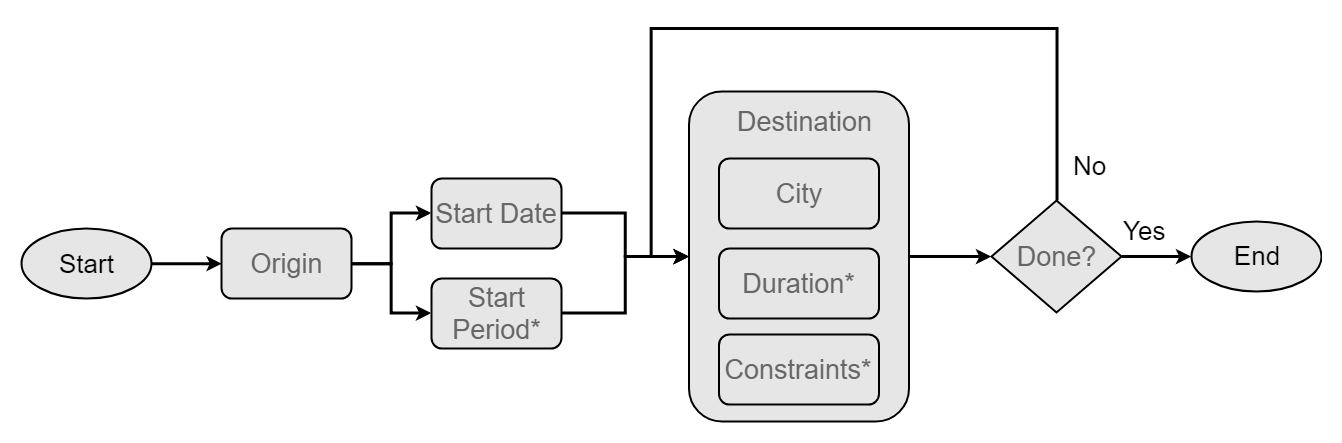
\includegraphics[width=\textwidth]{Figures/system_implementation/user_input.png}
%   \caption{Block diagram of the user input cycle.}
%   \label{fig:user_input}  
% \end{figure}


%_________________ AIRPORT VALIDATION ______________

% Figure of airport validation.
% This is not a central key to the program, so use the image only if we need extra content
% \begin{figure}[H]
%   \centering
%   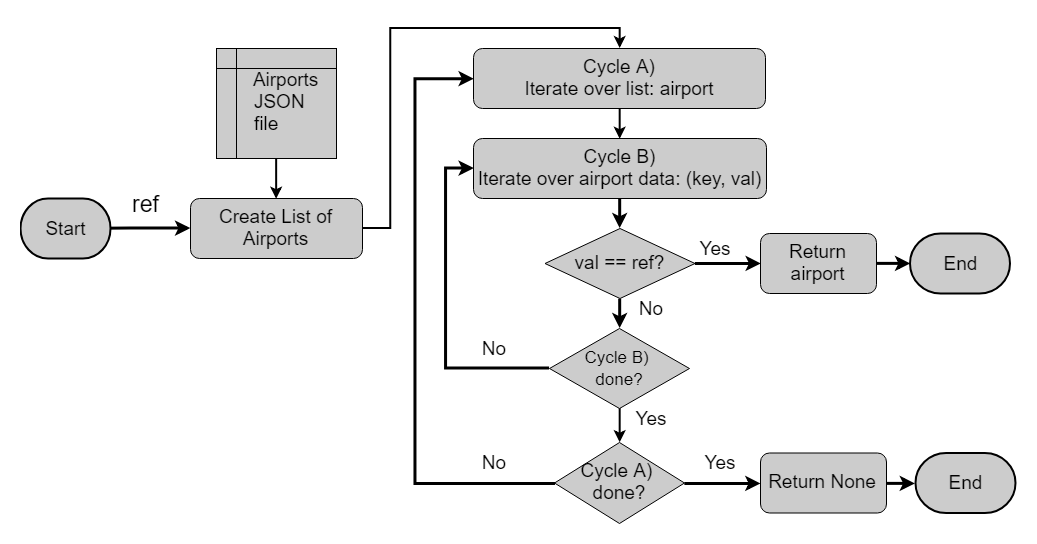
\includegraphics[width=\textwidth]{Figures/system_implementation/airports.png}
%   \caption{Validation of an user introduced airport based on an airport list stored in a JSON file.}
%   \label{fig:airports}  
% \end{figure}